%%%%%%%%%%%%%%%%%%%%%%%%%%%%%%%%%%%%%%%%%%%%%%%%%%%%%%%%%%%%
%  This is the generic Beamer for Ryan McWay's presentations
%%%%%%%%%%%%%%%%%%%%%%%%%%%%%%%%%%%%%%%%%%%%%%%%%%%%%%%%%%%%

% Declaring document as beamer with attributes
\documentclass[xcolor = x11names, compress, aspectratio = 169]{beamer}
% Settings for appearance of \pause
\setbeamercovered{transparent}

%%%%%%%%%%%%%%%%  Dependencies %%%%%%%%%%%%%%%%%%%%%%%
% Resize Figures
\usepackage{graphicx}
% Make Tables Fit Beamer Slide
\usepackage{booktabs}
\newcommand{\tinytable}[1]{\textcolor{black}{\tiny \input{#1} }}
% Make Drawings
\usepackage{tikz}
\usetikzlibrary{decorations.fractals}
% Allows to put greek letters outside of equations
\usepackage{textgreek}
% Bibliography Style
\usepackage[round]{natbib}
% Change Text Color 
\usepackage[dvipsnames]{xcolor}

% Allow to Color in Tables
\usepackage{colortbl}
\usepackage{threeparttable}
% Allow for PDFs in Latex Document
    \usepackage{pdfpages}

% Modelsumary requirements
\usepackage{tabularray}
\usepackage{float}
\usepackage[normalem]{ulem}
\UseTblrLibrary{booktabs}
\UseTblrLibrary{siunitx}
\newcommand{\tinytableTabularrayUnderline}[1]{\underline{#1}}
\newcommand{\tinytableTabularrayStrikeout}[1]{\sout{#1}}
\NewTableCommand{\tinytableDefineColor}[3]{\definecolor{#1}{#2}{#3}}

% Math font 
\usefonttheme[onlymath]{serif}

% Remove Beamer Toggle bar 
\beamertemplatenavigationsymbolsempty

% Define the ``official'' UMN colors
\xdefinecolor{GopherMaroon}{HTML}{7A0019}
\xdefinecolor{GopherGold}{HTML}{FFCC33}
\xdefinecolor{GopherLightGold}{HTML}{FFDE7A}
\xdefinecolor{GopherDarkMaroon}{HTML}{5B0013}

%%%%%%%%%%%%%%%%%%%%%%%%%%%%%%%%%%%%%%%%%%%%%%%%%%%%%%

%%%%%%%%%%%%%%%% Beamer Layout %%%%%%%%%%%%%%%%%%%%%%
\useoutertheme[subsection = false, shadow]{miniframes}
\useinnertheme{default}
\usefonttheme{structureitalicserif}
\usepackage{palatino}
\definecolor{mypurple}{rgb}{.49,0,98}
\setbeamerfont{title like}{shape = \scshape}
\setbeamerfont{frametitle}{shape = \scshape}


\setbeamercolor*{lower separation line head}{bg = GopherMaroon} 
\setbeamercolor*{normal text}{fg = black,bg = white} 
\setbeamercolor*{alerted text}{fg = GopherDarkMaroon} 
\setbeamercolor*{example text}{fg = black} 
\setbeamercolor*{structure}{fg = GopherDarkMaroon} 

\setbeamercolor*{palette tertiary}{fg = GopherMaroon,bg = black!10} 
\setbeamercolor*{palette quaternary}{fg = black,bg = black!10} 

\renewcommand{\(}{\begin{columns}}
\renewcommand{\)}{\end{columns}}
\newcommand{\<}[1]{\begin{column}{#1}}
\renewcommand{\>}{\end{column}}

% Allows for Gifs
\usepackage{animate}

% Allows for Appendix Frames
\usepackage{appendixnumberbeamer}

% Specify Frame Number in Footer
\setbeamertemplate{footline}
{
    \leavevmode %
    \hbox{%
        \begin{beamercolorbox}[wd = .333333\paperwidth, ht = 2.25ex, dp = 1ex, center]{Author Footer} %
            % \usebeamerfont{Author Footer}\insertshortauthor{}
            McWay, Gallagher
        \end{beamercolorbox}
        %
        \begin{beamercolorbox}[wd = .333333\paperwidth, ht = 2.25ex, dp = 1ex, center]{Title Footer} %
            % \usebeamerfont{Title Footer}\insertshorttitle{}
            Law of the Minimum
        \end{beamercolorbox}
        %
        \begin{beamercolorbox}[wd = .333333\paperwidth, ht = 2.25ex, dp = 1ex, right]{Date Footer} %
            \usebeamerfont{Date Footer}\today \hspace*{2em}
            \insertframenumber{} / \inserttotalframenumber\hspace*{2ex} 
        \end{beamercolorbox}}
        %
        \vskip0pt %
    }

% Hyperlink Colors
\hypersetup{
    colorlinks,
    citecolor = GopherMaroon,
    linkcolor = black
}

%%%%%%%%%%%%%%%%%%%%%%%%%%%%%%%%%%%%%%%%%%%%%%%%%%

%\beamerdefaultoverlayspecification{<+->}
\begin{document}

%%%%%%%%%%%%%%%%%%%%%%%%%%%%%%%%%%%%%%%%%%%%%%%%%%%%%%
%                Title Frame
%%%%%%%%%%%%%%%%%%%%%%%%%%%%%%%%%%%%%%%%%%%%%%%%%%%%%%
%\section{\scshape Introduction}

\begin{frame}
    \fontfamily{cmr}
    \title[Law of the Minimum]{
    Soil Capital for Crop Production: \\ Law of the Minimum}
    \author[McWay]{ 
        Ryan McWay$^\dagger$ \and 
        Nicholas Gallagher
    }
    \date{
    	NatCap TEEMs \\ 
    	\small{University of Minnesota} \\
    	\small{\textit{March 23rd, 2026}}
    }
    \institute[\textit{UMN}]{
        $^\dagger$\textit{Applied Economics, \\ 
        University of Minnesota}
    }
    
    \titlepage
\end{frame}

%%%%%%%%%%%%%%%%%%%%%%%%%%%%%%%%%%%%%%%%%%%%%%%%%%%%%%
%%%%%%%%%%%%%%%%%%%%%%%%%%%%%%%%%%%%%%%%%%%%%%%%%%%%%%

%%%%%%%%%%%%%%%%%%%%%%%%%%%%%%%%%
%      Motivation
%%%%%%%%%%%%%%%%%%%%%%%%%%%%%%%%%
\section{Motivation}
    \begin{frame}
    \fontfamily{cmr}
    \frametitle{Agriculture's Challenges}
        \begin{itemize}
            \item Farmers face two major challenges
            \item A necessity to sequester carbon and methane emissions amassing one third of global emissions contributing to climate change. {\scriptsize\citep{Vermeulen2012, Crippa2021}} 
            \begin{itemize}
                \item While we are making transitions in the energy sector and transportation, limited change in agriculture.
            \end{itemize}
            \item Modern field management has depleted the macro-nutrients for soil health resulting in soil degradation and soil erosion {\scriptsize\citep{Lal2015, Louwagie2009, Montgomery2007, Jie2002}} 
            \begin{itemize}
                \item Over extraction of the land leaves farmers more vulnerable to climatic shocks (i.e., the American Dust Bowl).
            \end{itemize}
        \end{itemize}
    \end{frame}
    %
    \begin{frame}
    \fontfamily{cmr}
    \frametitle{Soil Capital: Natural Capital vs. Agrochemicals}
        \begin{itemize}
            \item We conjecture that soil capital, the natural capital of the soil, is a key input for crop production and a potential substitute for agrochemical inputs.
            \item Soil capital is a stock of nutrients, organic matter, and microbial life that supports plant growth and ecosystem services.
            \item Agrochemicals are synthetic inputs such as fertilizers, pesticides, and herbicides that enhance crop growth and protect against pests and diseases.
            \begin{itemize}
                \item While agrochemicals can boost yields in the short term, they can also degrade soil health and reduce long-term productivity.
                \item Nitrogen fertilizer is the most widely used agrochemical input for crop production, but it also contributes to greenhouse gas emissions and water pollution. 
            \end{itemize}
            \item The law of the minimum states that crop yield is limited by the scarcest input, which may be soil capital or agrochemicals. {\scriptsize\citep{Brisson2010}}
            \begin{itemize}
                \item If soil capital is the limiting factor, then farmers can increase yields by investing in soil health rather than increasing agrochemical inputs.
            \end{itemize}
        \end{itemize}
    \end{frame}
    %
    % \begin{frame}
    % \fontfamily{cmr}
    % \frametitle{Regenerative Agriculture}
    %     \begin{itemize}
    %         \item The nascent concept of regenerative agriculture (RA) has promise in addressing both concerns {\scriptsize\citep{Paustian2016, LaCanne2018}}
    %         \item A wide set of practices budding from the sustainable agriculture movement, RA practices are primarily aimed at reducing chemical inputs, minimizing disturbance of the soil, and integrating ecosystems into farmer plots. 
    %         \item I focus on three related to carbon sequestration: 
    %         \begin{itemize}
    %             \item Cover cropping 
    %             \item No till
    %         \end{itemize} 
    %         \item While there is evidence that these practices sequester carbon at small scale, it is unclear if they are profitable for adoption. {\scriptsize\citep{Ogle2019, Wood2021, Nunes2018, Briske2011, Briske2008, Bosch2008}}
    %     \end{itemize}
    % \end{frame}
    % %
    \begin{frame}
    \fontfamily{cmr}
    \frametitle{Research Questions}
        \begin{block}{Research Questions}
            \begin{enumerate}
            \item Can we estimate the shifts in crop yields using soil capital as an input?
            \begin{itemize}
                \item Does it follow a CES production function or law of the minimum specification?
            \end{itemize}
            \item What is the tradeoff between soil capital and agrochemical inputs?
            \end{enumerate}
        \end{block}
    \end{frame}
    %
    % \begin{frame}
    % \fontfamily{cmr}
    % \frametitle{This Paper}
    %     \begin{enumerate}
    %         \item 
    %     \end{enumerate}
    % \end{frame}

%%%%%%%%%%%%%%%%%%%%%%%%%%%%%%%%%
%      Data
%%%%%%%%%%%%%%%%%%%%%%%%%%%%%%%%%
\section{Data}
    %
    \begin{frame}
    \fontfamily{cmr}
    \frametitle{Data}
    \begin{itemize}
        \item UW Forage and Soil Lab's WIDATCP certified labs soil summaries
        \begin{itemize}
            \item County-year panel for Wisconsin (1995--2017)
            \item Mean organic matter (OM, \%)
        \end{itemize}
        \item USDA NASS county corn grain yield (bu/acre) (1997 - 2017)
        \item Nitrogen fertilizer (1987 - 2017)
    \end{itemize}
    \end{frame}
    %
%%%%%%%%%%%%%%%%%%%%%%%%%%%%%%%%%
%      Production Functions
%%%%%%%%%%%%%%%%%%%%%%%%%%%%%%%%%
\section{Production Functions}
    %
    \begin{frame}
    \fontfamily{cmr}
    \frametitle{Production Functions}
        \begin{itemize}
            \item There are two reasonable specifications we may expect to model agricultural production. 
        \end{itemize}
        \begin{enumerate}
            \item Constant Elasticity of Substitution (CES) Production Function:
            \begin{itemize}
                \item Common in economics literature as a flexible functional form that nests both perfect substitutes and perfect complements. 
                \item However, it may not capture the nonlinearities in the yield response to inputs, especially if there are threshold effects or diminishing returns. 
            \end{itemize}
            \item Mitcherlich-Baule (Law of the Minimum) Specification:
            \begin{itemize}
                \item More consistent with agronomic theory and empirical evidence that crop yield is limited by the scarcest input. 
                \item However, it may be more difficult to estimate and interpret, especially if there are interactions between inputs or unobserved heterogeneity across farms.
            \end{itemize}
        \end{enumerate}
    \end{frame}
    %
    \begin{frame}
    \fontfamily{cmr}
    \frametitle{Inputs}
    \begin{itemize}
        \item Setting: Corn production in Wisconsin
        \item Objective: Per Acre Corn Yields 
        \item Key Inputs:
        \begin{itemize}
            \item Soil Capital: Mean Organic Matter (OM, \%)
            \begin{itemize}
                \item Ideal Level: 3-5\%, but many farmers have less than 2\% OM. {\scriptsize\citep{UMNExtSOM, UWExtA3588}}
            \end{itemize}
            \item Agrochemical Input: Nitrogen fertilizer per planted corn acre
            \begin{itemize}
                \item Ideal Level: 180 - 250 lbs/acre, but many farmers apply more than 300 lbs/acre. {\scriptsize\citep{NASS2022Corn, ERSFertilizer}}
            \end{itemize}
        \end{itemize}
    \end{itemize}
    \end{frame}
    %
        \begin{frame}
    \fontfamily{cmr}
    \frametitle{Wisconsin Data and Outcome}
        \begin{itemize}
            \item County-year panel for Wisconsin (1995--2017)
            \item Outcome: county corn grain yield (bu/acre)
            \item Soil covariate: mean organic matter (OM, \%)
            \item Fertilizer covariate: nitrogen per planted corn acre
            \item Final nonlinear sample: 1,415 observations across 65 counties
            \item Estimation via nonlinear least squares (Levenberg--Marquardt)
        \end{itemize}
    \end{frame}
    %
    \begin{frame}
    \fontfamily{cmr}
    \frametitle{CES Specification}
    \begin{itemize}
        \item Constant Elasticity of Substitution (CES) Specification:
        \begin{equation}
            y_{ct} = A_{ct}\left[\delta K_{ct}^{-\rho} + (1-\delta)N_{ct}^{-\rho}\right]^{-\frac{1}{\rho}}
        \end{equation}
        \item OM shifters:
        \begin{equation}
            A_{ct} = \alpha_0 + \alpha_1 OM_{ct}, \quad
            K_{ct} = \beta_0 + \beta_1 OM_{ct}
        \end{equation}
        \item Parameter interpretation:
        \begin{itemize}
            \item $A_{ct}$: Hicks-neutral productivity shifter
            \item $K_{ct}$: effective capital/input composite shifted by $OM_{ct}$
            \item $N_{ct}$: second input in the CES aggregator
            \item $\delta \in (0,1)$: share parameter between inputs
            \item $\rho = \frac{\sigma - 1}{\sigma}$, so $\sigma = \frac{1}{1+\rho}$ is the elasticity of substitution
        \end{itemize}
    \end{itemize}
    \end{frame}
    %
    
    \begin{frame}
    \fontfamily{cmr}
    \frametitle{CES Specification}
        \centering
        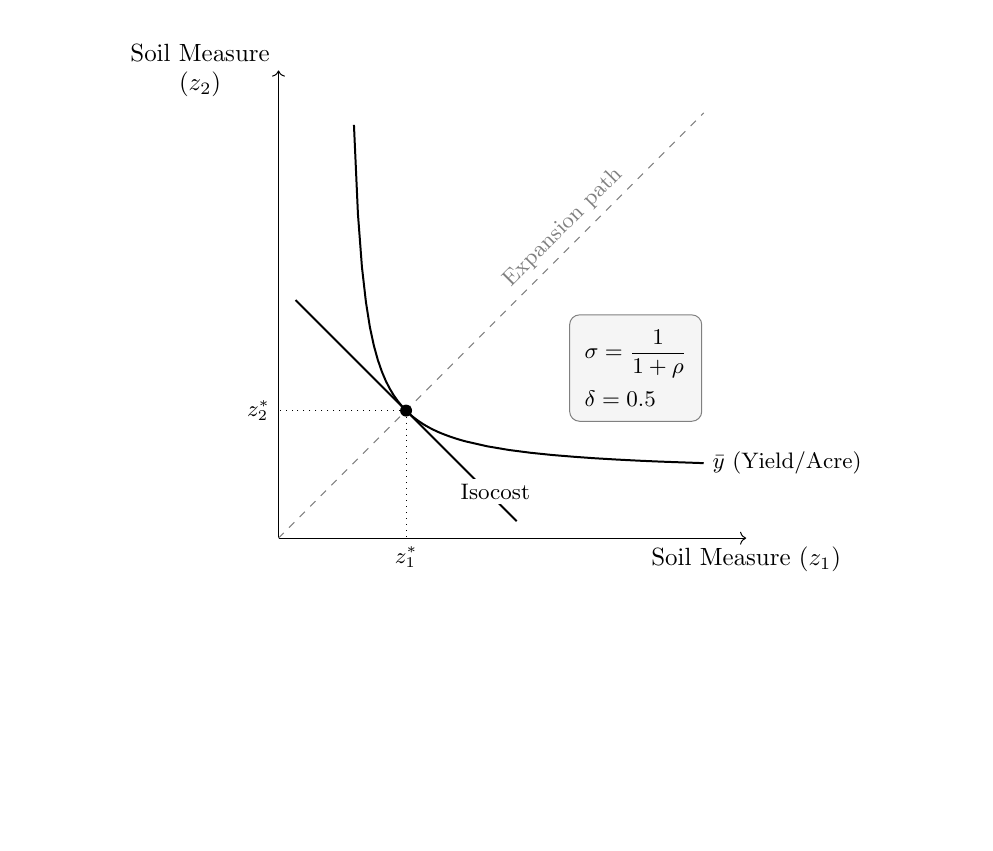
\includegraphics[width = 0.9\textwidth]{../output/images/figure-ces.png}
    \end{frame}
    %
    \begin{frame}
    \fontfamily{cmr}
    \frametitle{Law of the Minimum (LOM) Specification}
    \begin{itemize}
        \item Mitcherlich-Baule (Liebig's Law of the Minimum) Specification:
    \end{itemize}
    \begin{equation}    
        y_{ct} = \alpha_{ct} \left(1 - \beta_{ct} \exp(-\gamma X) \right)
    \end{equation}
    \begin{itemize}
        \item Specific Specification:
    \end{itemize}
    \begin{equation}    
        y_{ct} = A_{ct}\!\left[1 - B_{ct}\,\exp\!\left(-C_{ct}\, N_{ct}\right)\right]
    \end{equation}
    \begin{equation*}
        A_{ct} = \alpha_0 + \alpha_1 OM_{ct}, \quad
        B_{ct} = \beta_0 + \beta_1 OM_{ct}, \quad
        C_{ct} = e^{\gamma_0 + \gamma_1 OM_{ct}}
    \end{equation*}
    \begin{itemize}
        \item where $X \in \{OM, N\}$ is the input subject to diminishing returns
        \item $\alpha_{ct}$ is the baseline yield potential, $\beta_{ct}$ is the plateau parameter, and $\gamma$ is the decay rate of the yield response to $X$.
        \item The law of the minimum implies that yield is limited by the scarcest input, which may be soil capital or agrochemicals.
    \end{itemize}
    \end{frame}
    %
    \begin{frame}
    \fontfamily{cmr}
    \frametitle{LOM Specification}
        \centering
        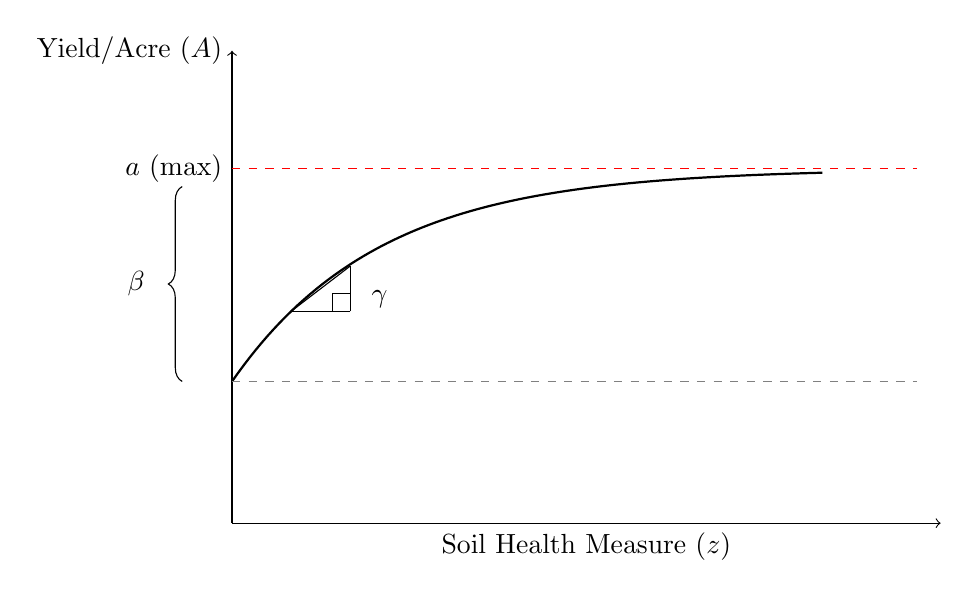
\includegraphics[width = 0.9\textwidth]{../output/images/figure-law-minimum.png}
    \end{frame}
    %
%%%%%%%%%%%%%%%%%%%%%%%%%%%%%%%%%
%          Results: CES
%%%%%%%%%%%%%%%%%%%%%%%%%%%%%%%%%
\section{Results: CES}
    %
    \begin{frame}[fragile]
    \fontfamily{cmr}
    \frametitle{CES Parameter Estimates}
        \begin{table}[!htbp]
\centering
\caption{CES Model Parameter Estimates for Wisconsin Corn Yield}
\label{tab:wi_ces_params}
\small
\resizebox{\textwidth}{!}{%
\begin{tabular}{llrrrrrr}
\toprule
Parameter & Interpretation & Estimate & Std. Error & t-value & p-value & 95\% CI Low & 95\% CI High \\
\midrule
$\alpha_0$ & Baseline Yield Shifter (bu/acre) & 111.17220 & 25691342.08155 & 0.000 & 1.0000 & -50354919.30765 & 50355141.65204 \\
$\alpha_1$ & Yield Shifter Sensitivity to OM & -4.31681 & 997593.79038 & -0.000 & 1.0000 & -1955288.14595 & 1955279.51233 \\
$\beta_0$ & Capital Composite Intercept & 1.01481 & 236175.68712 & 0.000 & 1.0000 & -462903.33194 & 462905.36156 \\
$\beta_1$ & Capital Composite Sensitivity to OM & 0.13561 & 31561.29698 & 0.000 & 1.0000 & -61860.00646 & 61860.27769 \\
$d$ (logit $\delta$) & Logit Share Parameter (logit $\delta$) & 4.95164 & 816552.60433 & 0.000 & 1.0000 & -1600438.15285 & 1600448.05613 \\
$\rho$ & Substitution Parameter & 3.50859 & 1.28815 & 2.724 & 0.0065 & 0.98381 & 6.03338 \\
\bottomrule
\end{tabular}
}
\begin{tablenotes}[flushleft]
\footnotesize
\item Notes: Derived $\delta = 0.9930$ (input share), $\sigma = 0.2218$ (elasticity of substitution). $\delta$ recovered via $\delta = 1/(1+e^{-d})$.
\end{tablenotes}
\end{table}

    \end{frame}
    %
    \begin{frame}
    \fontfamily{cmr}
    \frametitle{CES Model Fit Summary}
        \begin{itemize}
            \item Pseudo-$R^2$: 0.0576
            \item RMSE: 23.92
            \item Residual SE: 23.97
            \item Derived $\delta = 0.993$ (share weight on $K$); derived $\sigma = 0.222$ (elasticity of substitution)
            \item Most parameters are statistically insignificant; model is poorly identified
        \end{itemize}
    \end{frame}
    %
    \begin{frame}
    \fontfamily{cmr}
    \frametitle{CES Results Visualized}
        \centering
        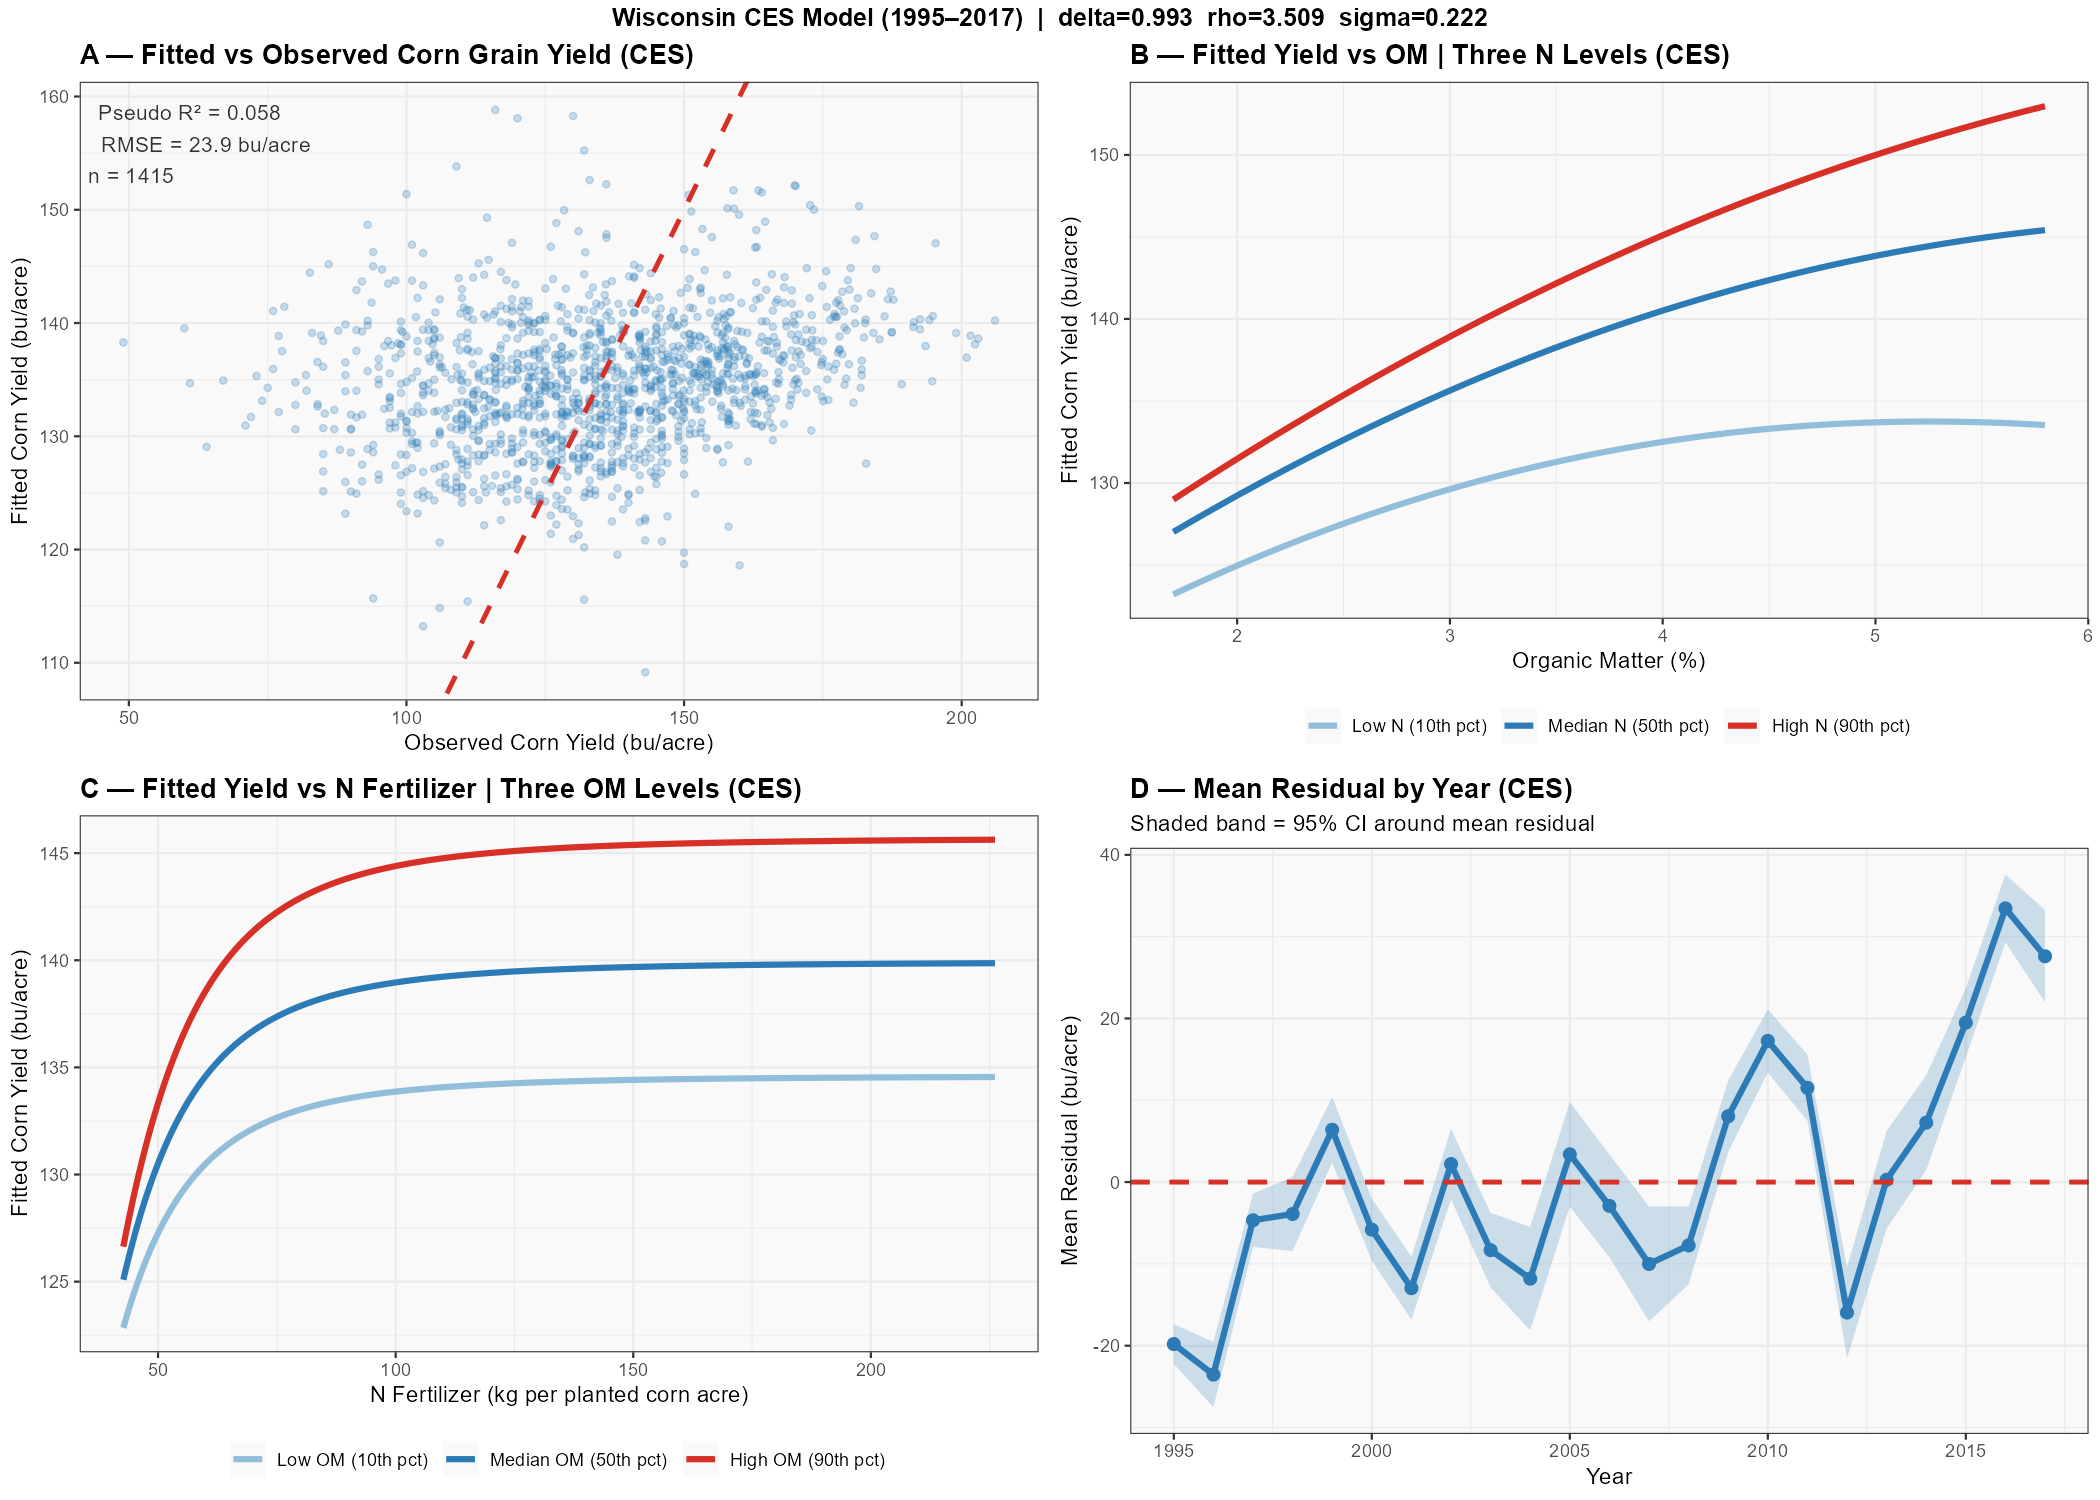
\includegraphics[width = 0.7\textwidth]{../output/figures/figure_wi_ces_visuals.png}
    \end{frame}
    %
    \begin{frame}
    \fontfamily{cmr}
    \frametitle{CES OM--N Tradeoff Contours}
        \centering
        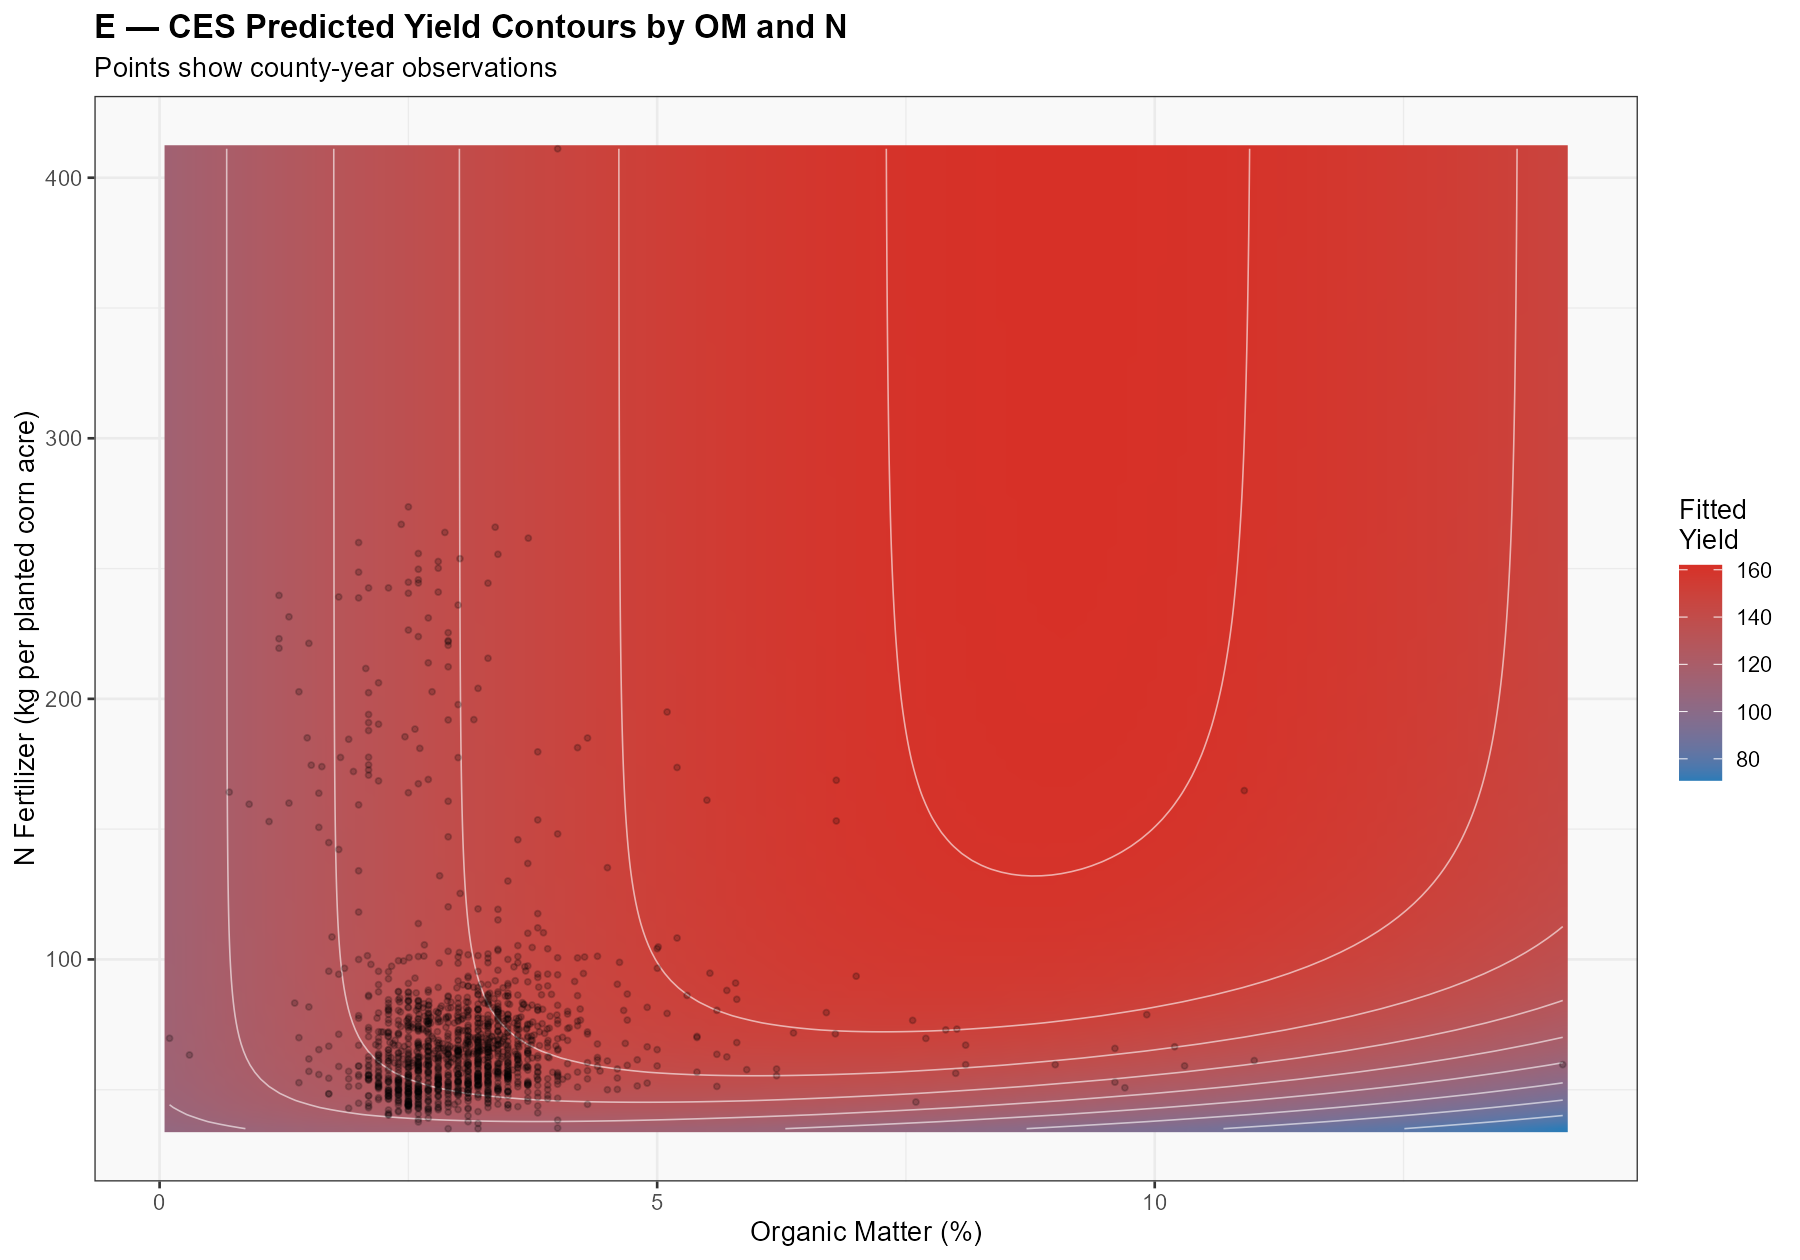
\includegraphics[width = 0.7\textwidth]{../output/figures/figure_wi_ces_contour_om_n.png}
    \end{frame}
    %
%%%%%%%%%%%%%%%%%%%%%%%%%%%%%%%%%
%          Results: LOM
%%%%%%%%%%%%%%%%%%%%%%%%%%%%%%%%%
\section{Results: LOM}
    %
    \begin{frame}[fragile]
    \fontfamily{cmr}
    \frametitle{LOM Parameter Estimates}
        \begin{table}[!htbp]
\centering
\caption{Model Parameter Estimates for Wisconsin Corn Yield}
\label{tab:wi_model_params}
\small
\resizebox{\textwidth}{!}{%
\begin{tabular}{llccccccc}
\toprule
Parameter & Interpretation & Estimate & Std. Error & t-value & p-value & 95\% CI Low & 95\% CI High \\
\midrule
$\alpha_0$ & Baseline Yield (bu/acre) & 139.74030 & 3.45959 & 40.392 & 0.0000 & 132.95951 & 146.52109 \\
$\alpha_1$ & Yield increase per 1\% OM & 0.06846 & 0.81697 & 0.084 & 0.9332 & -1.53279 & 1.66971 \\
$\beta_0$ & Decay Plateau Parameter & 0.40676 & 0.21534 & 1.889 & 0.0591 & -0.01530 & 0.82883 \\
$\beta_1$ & Decay Plateau Sensitivity to OM & 0.05840 & 0.12644 & 0.462 & 0.6442 & -0.18942 & 0.30623 \\
$\gamma_0$ & Decay Rate (log scale) & -0.79374 & 0.60224 & -1.318 & 0.1877 & -1.97413 & 0.38665 \\
$\gamma_1$ & Decay Rate Sensitivity to OM & 0.80591 & 0.18322 & 4.398 & 0.0000 & 0.44679 & 1.16503 \\
\bottomrule
\end{tabular}
}
\begin{tablenotes}[flushleft]
\footnotesize
\item Notes: $\gamma_0$ and $\gamma_1$ are estimated on the log scale through $\gamma = \exp(\gamma_0 + \gamma_1 \cdot \text{OM})$.
\end{tablenotes}
\end{table}

    \end{frame}
    %
    \begin{frame}
    \fontfamily{cmr}
    \frametitle{LOM Model Fit Summary}
        \begin{itemize}
            \item Pseudo-$R^2$: 0.0648
            \item RMSE: 23.83 
            \item Residual SE: 23.88 
            \item Estimated decay sensitivity $\gamma_1 > 0$ and statistically significant
        \end{itemize}
    \end{frame}
    %
    \begin{frame}
    \fontfamily{cmr}
    \frametitle{LOM Results Visualized}
        \centering
        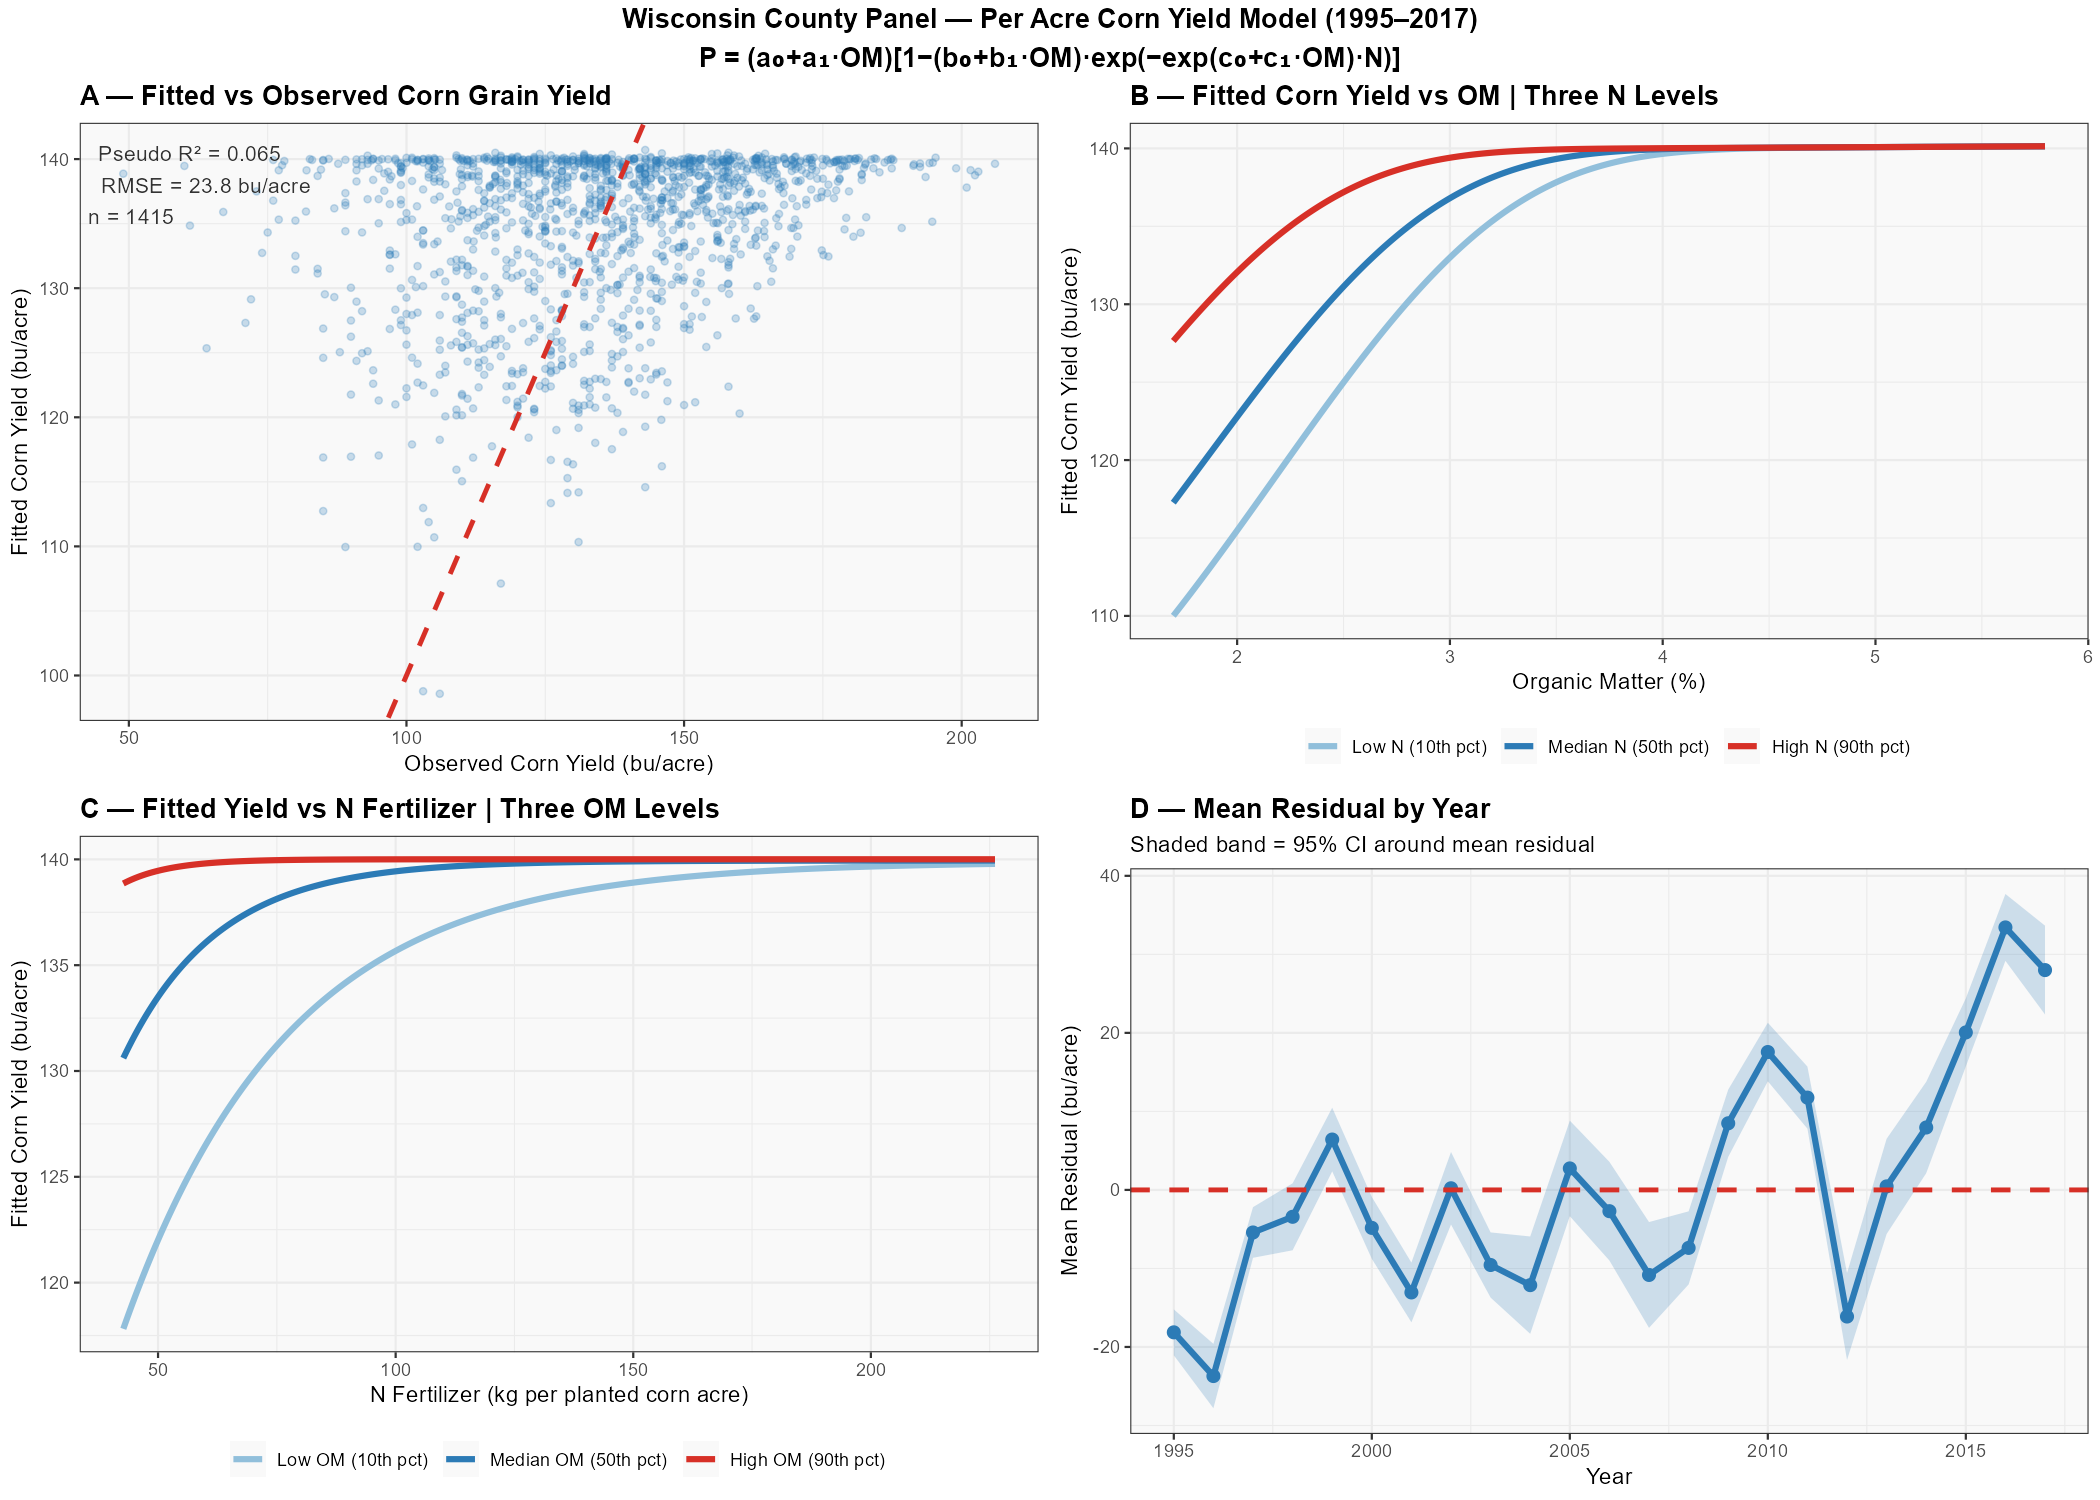
\includegraphics[width = 0.7\textwidth]{../output/figures/figure_wi_model_visuals.png}
    \end{frame}
    %
    % \begin{frame}
    % \fontfamily{cmr}
    % \frametitle{LOM Results Plot A: Fitted vs Observed}
    %     \centering
    %     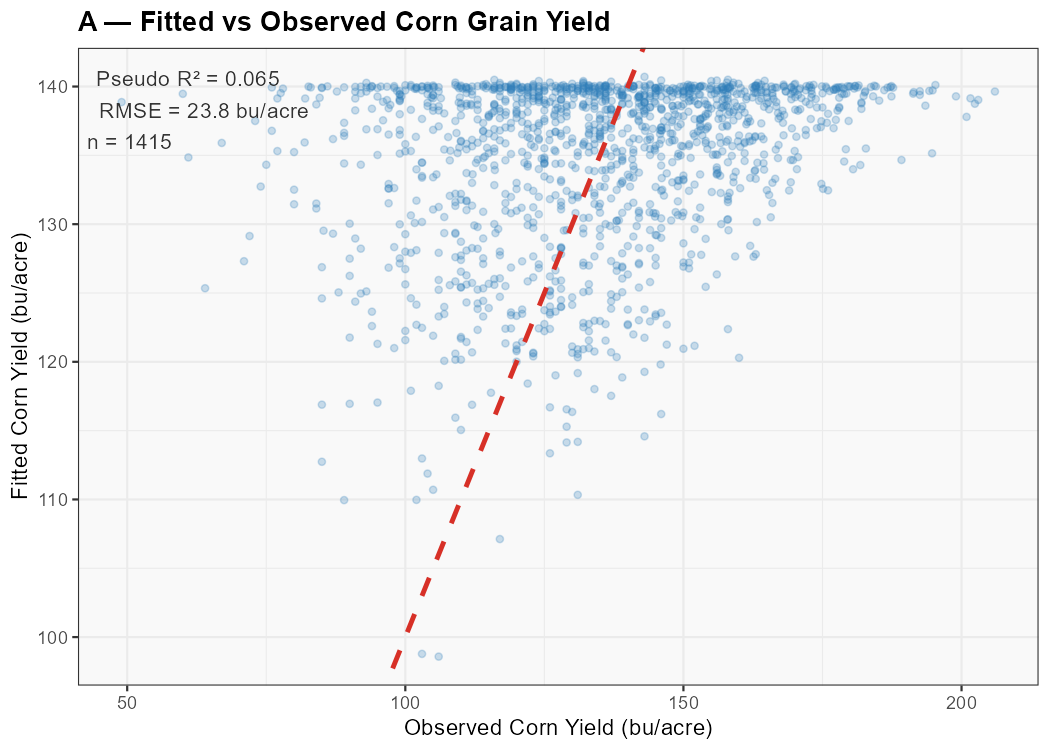
\includegraphics[width = 0.7\textwidth]{../output/figures/figure_wi_model_plot_A.png}
    % \end{frame}
    % %
    % \begin{frame}
    % \fontfamily{cmr}
    % \frametitle{LOM Results Plot B: Yield Response Over OM}
    %     \centering
    %     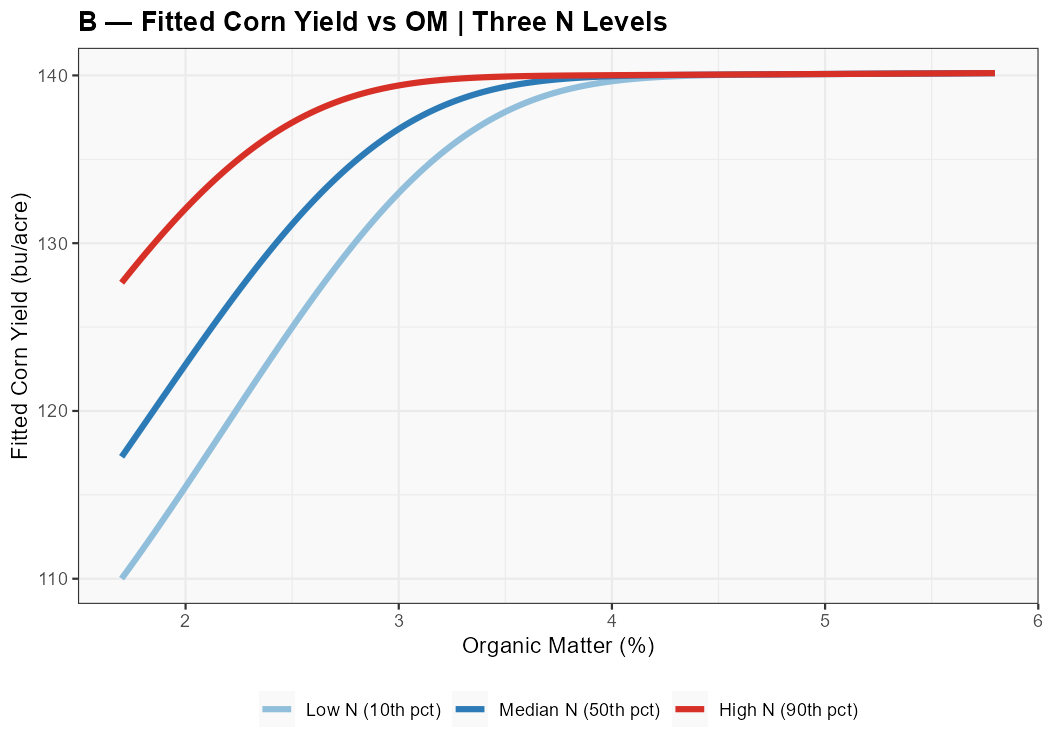
\includegraphics[width = 0.7\textwidth]{../output/figures/figure_wi_model_plot_B.png}
    % \end{frame}
    % %
    % \begin{frame}
    % \fontfamily{cmr}
    % \frametitle{LOM Results Plot C: Yield Response Over N}
    %     \centering
    %     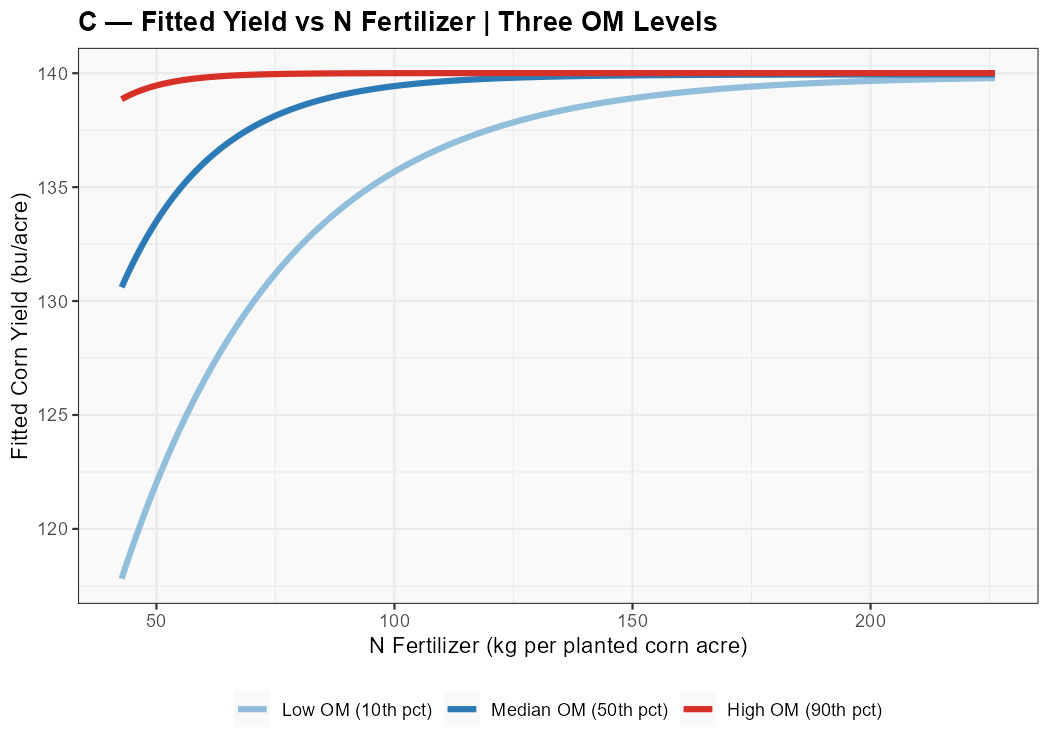
\includegraphics[width = 0.7\textwidth]{../output/figures/figure_wi_model_plot_C.png}
    % \end{frame}
    % %
    % \begin{frame}
    % \fontfamily{cmr}
    % \frametitle{LOM Results Plot D: Mean Residual by Year}
    %     \centering
    %     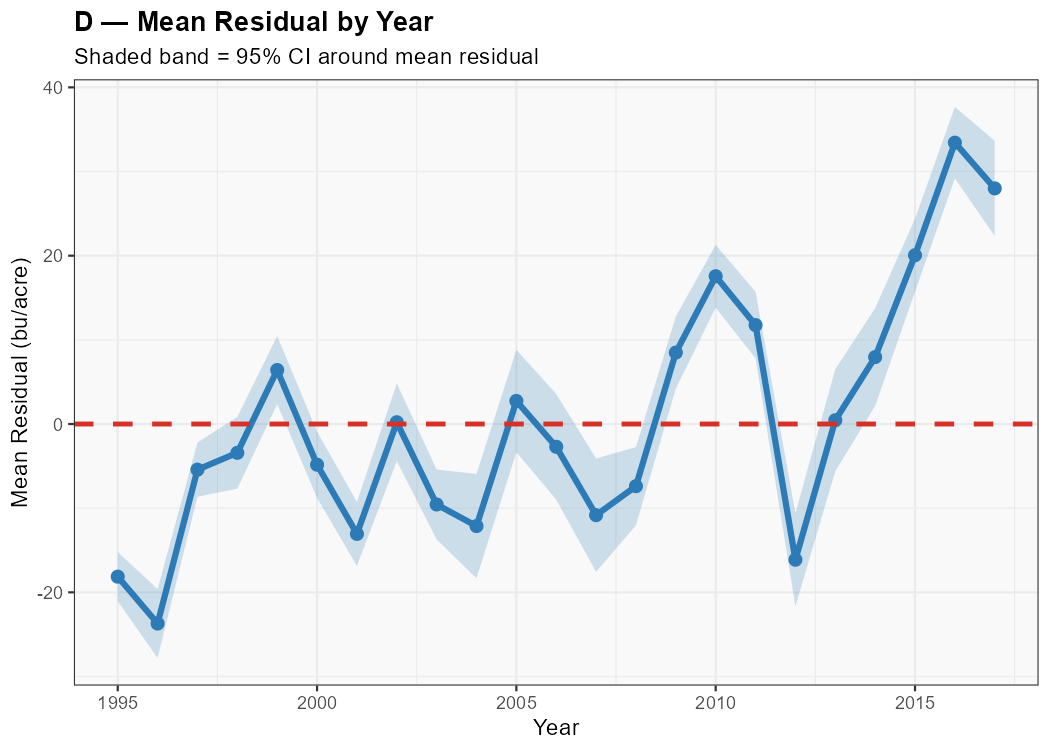
\includegraphics[width = 0.7\textwidth]{../output/figures/figure_wi_model_plot_D.png}
    % \end{frame}
    % %
    \begin{frame}
    \fontfamily{cmr}
    \frametitle{LOM OM--N Tradeoff Contours}
        \centering
        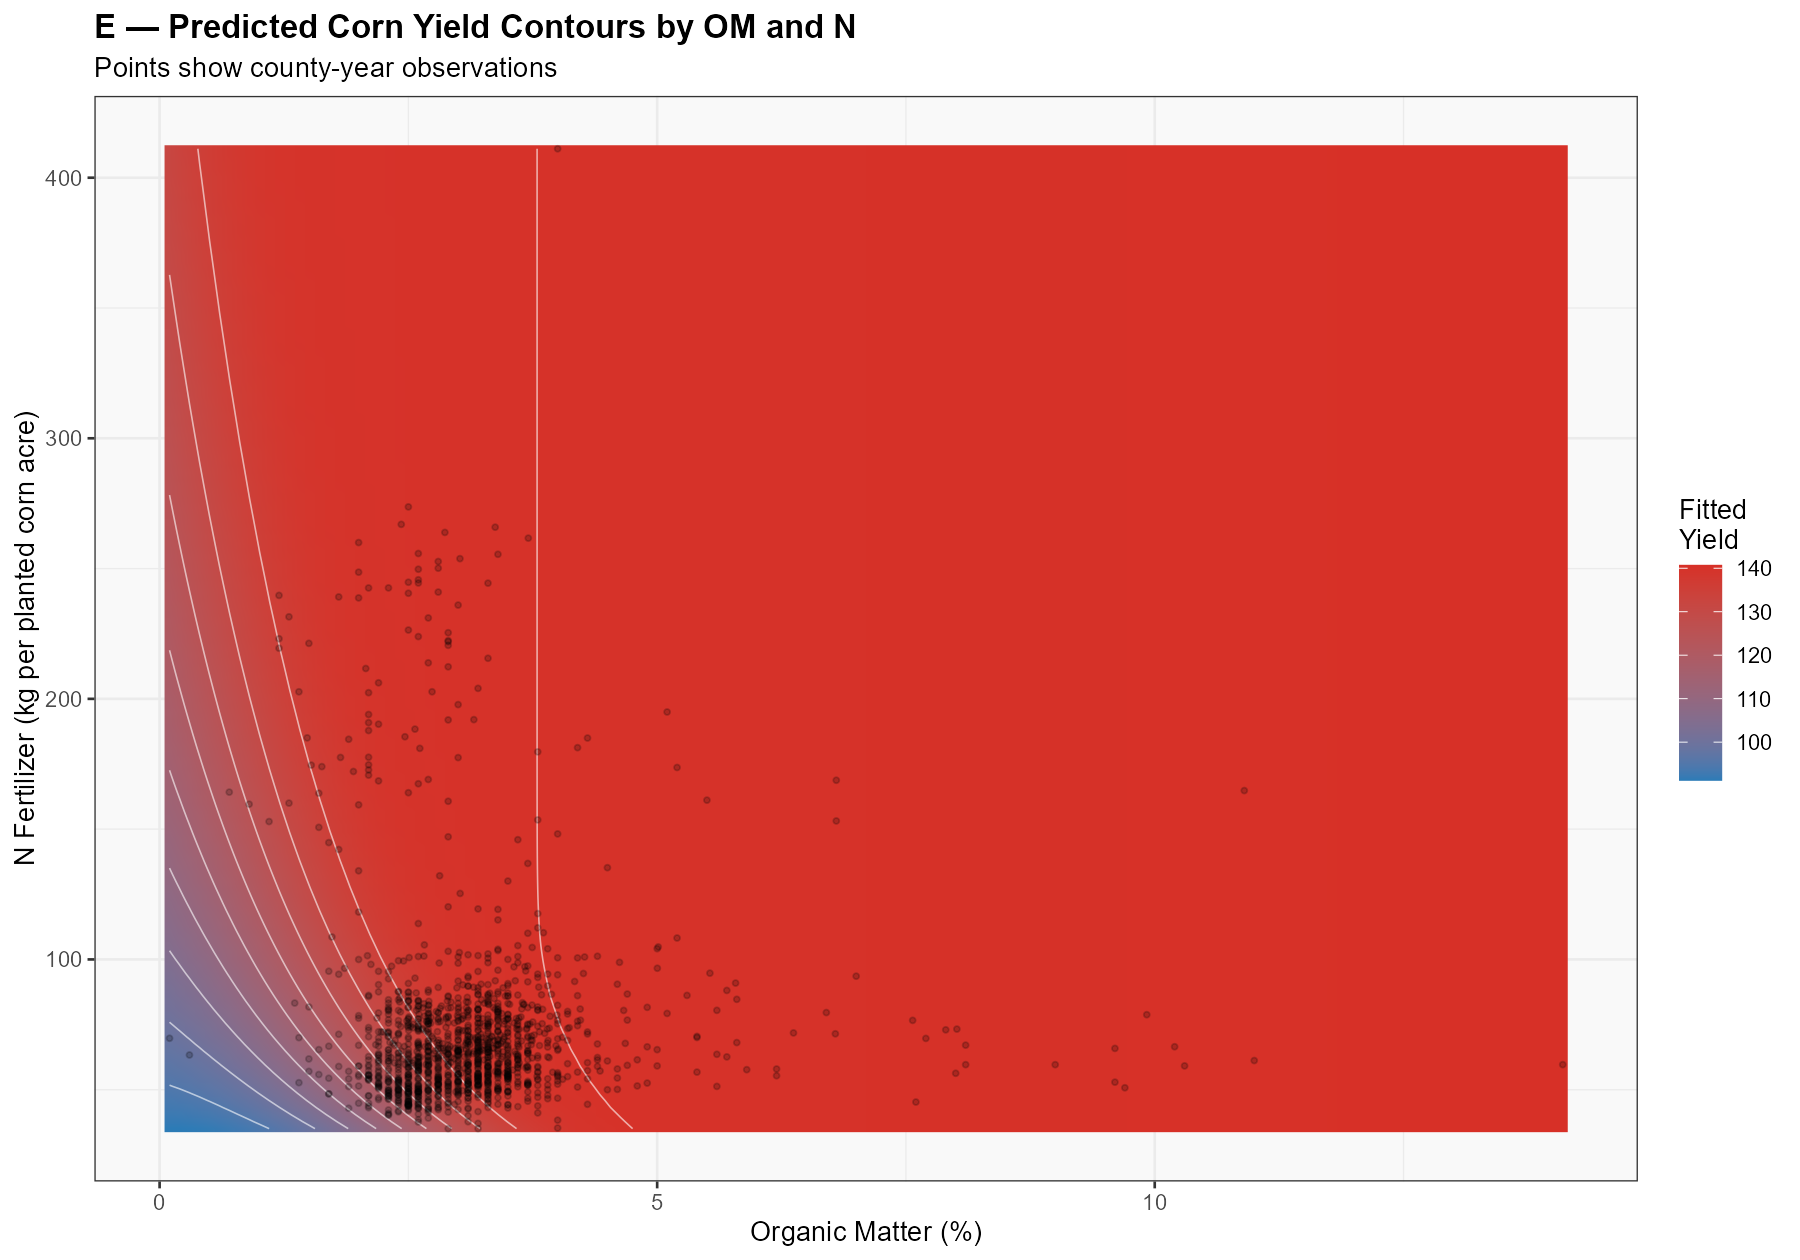
\includegraphics[width = 0.7\textwidth]{../output/figures/figure_wi_model_contour_om_n.png}
    \end{frame}
    %
%%%%%%%%%%%%%%%%%%%%%%%%%%%%%%%%%
%          Conclusions
%%%%%%%%%%%%%%%%%%%%%%%%%%%%%%%%%
\section{Conclusions}
    \begin{frame}[label = contributions]
    \fontfamily{cmr}
    \frametitle{Summary}
        \begin{itemize}
            \item Comparison of two production function specifications: CES and LOM
            \item LOM specification fits the data better and is more consistent with agronomic theory
            \item Tradeoff contours suggest that soil capital can substitute for agrochemical inputs, but the degree of substitution depends on the levels of both inputs and the yield response to them.
            \item The results have implications for farmers' decisions on how to invest in soil health and agrochemical inputs, as well as for policymakers' efforts to promote sustainable agriculture and reduce greenhouse gas emissions.
        \end{itemize}
    \end{frame}
    %      
    \begin{frame}[label = contributions]
    \fontfamily{cmr}
    \frametitle{Next Steps}
        \begin{itemize}
            \item Explore some other soil macronutrients (e.g., soil pH, Potasium, Phosphorus)
            \item Explore other crops and regions (e.g., soybeans, national state data)
            \item Explore influence of regenerative agriculture practices on soil capital and yields (e.g., cover cropping, no till)
        \end{itemize}
    \end{frame}
    %  
    \begin{frame}[label = conclusion]
    \fontfamily{cmr}
    \frametitle{The End}
        \centering 
        \Large{\emph{Thank You for Your Time!}} \\
        \hspace{1.5cm} \\
        \small{Contact: \textit{mcway005@umn.edu}} \\
        \small{Website: \textit{mcwayrm.github.io}}
    \end{frame}
    %
 
%%%%%%%%%%%%%%%%%%%%%%%%%%%%%%%%%
%           Appendix
%%%%%%%%%%%%%%%%%%%%%%%%%%%%%%%%%
% \appendix
%     %
%     \begin{frame}[label = alt. cover crop]
%     \fontfamily{cmr}
%     \frametitle{Cover Cropping Design}
%     \framesubtitle{\hyperlink{cover crop}{\beamerreturnbutton{Cover Crop}}}
%         \centering 
%         \includegraphics[width = .7\textwidth]{images/diagram-cover-crop-02.jpg}
%     \end{frame}

    
%%%%%%%%%%%%%%%%%%%%%%%%%%%%%%%%%
%           Bibliography
%%%%%%%%%%%%%%%%%%%%%%%%%%%%%%%%%

\begin{frame}[allowframebreaks, noframenumbering]
    \fontfamily{cmr}
    \frametitle{References}
    \footnotesize{
    \bibliographystyle{chicago}
    \bibliography{references.bib}
    }
\end{frame}

\end{document}